%   MSc Business Analytics Dissertation
%
%   Title:     Aaa Bbbbbbb Cccccccccc
%   Author(s): Xxxxxx Xxxxxxxxx and Yyy Yyyyyyyyy
%
%   Chapter 7: Conclusions and Future Research
%
%   Change Control:
%   When     Who   Ver  What
%   -------  ----  ---  --------------------------------------------------------------
%   11Feb11  AB    0.1  Begun 
%

\chapter{Conclusions and Future Research}\label{C.Conclusions.Future.research}

\section{Integration with real data}

Credit scoring is a senstive and important component of any bank and financial institutions. The outcome of this work presents a predictive model that connects with a business dashboard. One can integrate the day to day financial data from a bank with this dashboard. This work can be improvised with the help of real banking data so that predictive model can be trained efficiently.
\begin{description}
\item[Dashboard:] Real transactional data can improve the performance of Tableau dashboard which acts as decision support system 
\item[Geospatial Data:] Credit assessment can be enhanced if it includes information such as house coordinates
\item[External Factors:] The model can perform better when trained with large number of external factors such as medical information, average salary in neighbourhood

\end{description}

\section{Future Work}
\begin{center}
\begin{figure}[!htb]
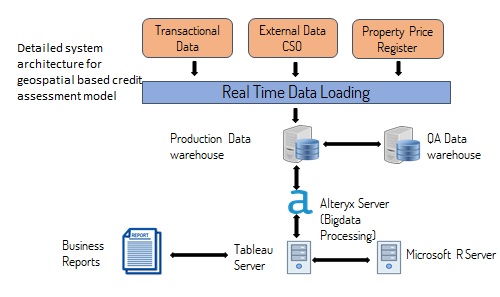
\includegraphics[width=\textwidth]{future.png}
\centering
\caption{System Architecture}{\textbf{Source:} MS Powerpoint}
\label{fig:future}
\end{figure}
\end{center}
\section{Conclusion}
The objective of this project was to build an interactive and efficient dashboard that supports credit analysis and assessment of residential loan portfolios with the help of geospatial methods. This practicum was stemmed on aggregation of loan portfolio data and financial services data that adheres to credit assessment policies and macroeconomic performance indicators. The purpose of developing predictive models for calculating the probability of default using logistic regression and decision trees was successfully achieved.  Initial review of the literature revealed that majority of the researchers believe models developed using logistic regression show better performance compared to decision trees regarding accuracy and area under ROC, but few have concluded the opposite. This practicum falls into the category of those researchers, who have stated decision trees give better performance than logistic regression based on KS, GINI and ROC statistics.  Although, because of the limitation of data, it cannot be said that the developed predictive model will show similar results when connected to real life dataset. There are possibilities that logistic regression can give better performance compared to decision trees.

